%% Author: Leighton Pritchard
%% Copyright: James Hutton Institute
%% 2015-03-07: Slides for teaching at University of Dundee, 17th March 2015
%% This presentation was an invited lecture on comparative genomics and visualisation
%% for the BS32010 course.

%% UNCOMMENT FOR SLIDES
\documentclass[table]{beamer}
\mode<presentation>

%% UNCOMMENT FOR HANDOUTS
%\documentclass[handout]{beamer}
\usepackage{handoutWithNotes}
\pgfpagesuselayout{4 on 1 with notes}[a4paper,border shrink=5mm]

%% GENERIC STYLE SETTINGS BELOW
\usetheme{default}
\usepackage{listings}
\usepackage{multirow}
\usepackage{xcolor}
\usepackage{hyperref}
%\usepackage[multiple]{footmisc}

\usebackgroundtemplate{

\includegraphics[width=\paperwidth,height=\paperheight]{images/hutton_background}
}
%% PRESENTATION CONFIGURATION PARAMETERS %%%%%%%%%%%%%%%%%%%%%%%%%%%%%%%%%%%%%%%
%\titlebackgroundfile{images/hutton_title}
%\framebackgroundfile{images/hutton_background}
\definecolor{hutton_green}{HTML}{78A22F}
\definecolor{hutton_purple}{HTML}{872175}
\definecolor{hutton_blue}{HTML}{569BBE}
\definecolor{olive}{rgb}{0.3, 0.4, .1}
\definecolor{fore}{RGB}{249,242,215}
\definecolor{back}{RGB}{51,51,51}
\definecolor{title}{RGB}{255,0,90}
\definecolor{dgreen}{rgb}{0.,0.6,0.}
\definecolor{gold}{rgb}{1.,0.84,0.}
\definecolor{JungleGreen}{cmyk}{0.99,0,0.52,0}
\definecolor{BlueGreen}{cmyk}{0.85,0,0.33,0}
\definecolor{RawSienna}{cmyk}{0,0.72,1,0.45}
\definecolor{Magenta}{cmyk}{0,1,0,0}
\usefonttheme{structurebold}
\setbeamercolor{alerted text}{fg=orange}
\setbeamercolor{background canvas}{bg=white}
\setbeamercolor{block title}{bg=hutton_purple}
\setbeamercolor{frametitle}{fg=hutton_purple}
\setbeamercolor{title}{fg=black}
\setbeamercolor{titlelike}{fg=hutton_green}
\setbeamercolor{author}{fg=hutton_purple}
\setbeamercolor{author in head/foot}{fg=white}
\setbeamercolor{title in head/foot}{fg=white}
\setbeamercolor{section in head/foot}{fg=hutton_purple}
\setbeamercolor{normal text}{fg=black}
\setbeamercolor{frametitle}{fg=hutton_purple}
\setbeamerfont{block title}{size={}}
\setbeamerfont{author}{size=\footnotesize}
\setbeamerfont{institute}{size=\tiny}
\setbeamerfont{date}{size=\footnotesize}
\setbeamercolor{section in toc shaded}{fg=hutton_purple}
\setbeamercolor{section in toc}{fg=hutton_purple}
\setbeamercolor{subsection in toc shaded}{fg=hutton_purple}
\setbeamercolor{subsection in toc}{fg=hutton_purple}
\setbeamertemplate{itemize item}[circle]
\setbeamertemplate{itemize subitem}[circle]
\setbeamertemplate{itemize subsubitem}[circle]
\setbeamertemplate{itemize subsubsubitem}[circle]
\setbeamercolor{itemize item}{fg=hutton_purple}
\setbeamercolor{itemize subitem}{fg=hutton_purple}
\setbeamercolor{itemize subsubitem}{fg=hutton_purple}
\setbeamercolor{itemize subsubsubitem}{fg=hutton_purple}
\setbeamercolor{enumerate item}{fg=hutton_purple}
\setbeamercolor{enumerate subitem}{fg=hutton_purple}
\setbeamercolor{enumerate subsubitem}{fg=hutton_purple}
\setbeamercolor{enumerate subsubsubitem}{fg=hutton_purple}
\setbeamercolor{alerted text}{fg=hutton_green}
\setbeamerfont{alerted text}{series=\bfseries}
% This command makes sure that acrobat reader doesn't change the colours of the slide
% when there are figures with transparencies.
\pdfpageattr {/Group << /S /Transparency /I true /CS /DeviceRGB>>}

%Disables discrete bottom navigation bar
\beamertemplatenavigationsymbolsempty

% Modify the slide titles to avoid the corner images,
\setbeamertemplate{frametitle}
{
\vspace{0.05\textheight}
\noindent\quad\begin{minipage}[t][0.12\textheight][t]{0.85\textwidth}
\insertframetitle\par
\end{minipage}
}

% Modify title page to avoid the big logo on right
\setbeamertemplate{title page}{
    \begin{picture}(0,0)
            %This ends up on top of the default background image, rather than replacing it:
            \put(-30,-165){%
                
\includegraphics[width=\paperwidth,height=\paperheight]{images/hutton_title}
            }
            \put(0,-75){%
                \begin{minipage}[b][0.4\textheight][t]{0.75\textwidth}
                    \usebeamerfont{title}\usebeamercolor[fg]{title}{\inserttitle\par}
                    \usebeamerfont{subtitle}\usebeamercolor[fg]{subtitle}{\insertsubtitle\par}
                \end{minipage}
            }
            \put(0,-125){%
                \begin{minipage}[b][0.1\textheight][t]{\textwidth}
                    \usebeamerfont{author}\usebeamercolor[fg]{author}{\insertauthor\par}
                    \usebeamerfont{institute}\usebeamercolor[fg]{institute}{\insertinstitute\par}
                \end{minipage}
            }
    \end{picture}
}

% Make \verbatim environment tiny font
\makeatletter
\def\verbatim{\tiny\@verbatim \frenchspacing\@vobeyspaces \@xverbatim}
\makeatother

%%%%%%%%%%%%%%%%%%%%%%%%%%%%%%%%%%%%%%%%%%%%%%%%%%%%%%%%%%%%%%%%%%%%%%%%%%%%%%%%

% LISTINGS SETTING
% Settings for code listings in lstlistings

\definecolor{hutton_lightgreen}{HTML}{C8F27F}

\lstset{ %
  backgroundcolor=\color{hutton_lightgreen},   % choose the background color; you must add \usepackage{color} or \usepackage{xcolor}
  basicstyle=\tiny\ttfamily,        % the size of the fonts that are used for the code
  breakatwhitespace=false,         % sets if automatic breaks should only happen at whitespace
  breaklines=true,                 % sets automatic line breaking
  captionpos=b,                    % sets the caption-position to bottom
  commentstyle=\color{red},    % comment style
  deletekeywords={...},            % if you want to delete keywords from the given language
  escapeinside={\%*}{*)},          % if you want to add LaTeX within your code
  extendedchars=true,              % lets you use non-ASCII characters; for 8-bits encodings only, does not work with UTF-8
  frame=single,                    % adds a frame around the code
  keepspaces=true,                 % keeps spaces in text, useful for keeping indentation of code (possibly needs columns=flexible)
  keywordstyle=\color{blue},       % keyword style
%  language=Octave,                 % the language of the code
  morekeywords={*,...},            % if you want to add more keywords to the set
  numbers=left,                    % where to put the line-numbers; possible values are (none, left, right)
  numbersep=5pt,                   % how far the line-numbers are from the code
  numberstyle=\tiny\color{gray}, % the style that is used for the line-numbers
  rulecolor=\color{black},         % if not set, the frame-color may be changed on line-breaks within not-black text (e.g. comments (green here))
  showspaces=false,                % show spaces everywhere adding particular underscores; it overrides 'showstringspaces'
  showstringspaces=false,          % underline spaces within strings only
  showtabs=false,                  % show tabs within strings adding particular underscores
  stepnumber=1,                    % the step between two line-numbers. If it's 1, each line will be numbered
  stringstyle=\color{violet},     % string literal style
  tabsize=4,                       % sets default tabsize to 2 spaces
  title=\lstname                   % show the filename of files included with \lstinputlisting; also try caption instead of title
}


%%%
% TITLE PREAMBLE
\title[Comparative Genomics and Visualisation: 4.Genome Features] % (optional, only for long titles)
{Comparative Genomics and \\ Visualisation \\
BS32010 \\
4.Genome Feature Comparisons}
%\subtitle{}
\author[Pritchard] % (optional, for multiple authors)
{Leighton~Pritchard$^{1,2,3}$}
\institute[The James Hutton Institute] % (optional)
{
  $^{1}$Information and Computational Sciences,\\
  $^{2}$Centre for Human and Animal Pathogens in the Environment,\\
  $^{3}$Dundee Effector Consortium,\\
  The James Hutton Institute, Invergowrie, Dundee, Scotland, DD2 5DA
}
\date[17th March 2015] % (optional)
{17th March 2015}
\subject{Bioinformatics, Genomics, Bacteria, Sequencing, Microbiology, Microbes, Comparative Genomics, Visualisation}

%%%
% TOC
% Show table of contents, with current section highlighted,
% at the start of each section

%\AtBeginSection[]
%{
%  \begin{frame}
%    \frametitle{Table of Contents}
%    \tableofcontents[currentsection] %,hideallsubsections]
%  \end{frame}
%}

\AtBeginSubsection[]
{
  \begin{frame}
    \frametitle{Table of Contents}
    \tableofcontents[currentsection,currentsubsection] %,hideallsubsections]
  \end{frame}
}

%%%
% START DOCUMENT
\begin{document}

\frame[plain]{\titlepage}

%% use.tex
%% Author: Leighton Pritchard
%% Copyright: James Hutton Institute
%% These slides describe the acceptable use policy for these slides and
%% materials

%
\begin{frame}
  \frametitle{Acceptable Use Policy}
  Recording of this talk, taking photos, discussing the content using \\
  email, Twitter, blogs, etc. is permitted (and encouraged), \\
  providing distraction to others is minimised. \\[0.5cm]
  These slides will be made available on SlideShare. \\[0.5cm]
  \textbf{These slides, and supporting material including exercises, are available at \href{https://github.com/widdowquinn/Teaching-2015-03-17-UoD_compgenvis}{https://github.com/widdowquinn/Teaching-2015-03-17-UoD\_compgenvis}}
\end{frame}

%%%
% SECTION: Comparisons of genome Features
\section{Comparisons of genome features}
% SUBSECTION
% Genome features
\subsection{Genome Features}
%% genome_features.tex
%% Author: Leighton Pritchard
%% Copyright: James Hutton Institute
%% Genome features

%
\begin{frame}
  \frametitle{Gene features}
  \textcolor{hutton_green}{Genes:}
  \begin{columns}[T] 
    \column{.4\textwidth} 
      \begin{itemize}
        \item translation start
        \item introns
        \item exons
        \item translation stop
        \item translation terminator
      \end{itemize}
    \column{.6\textwidth}
      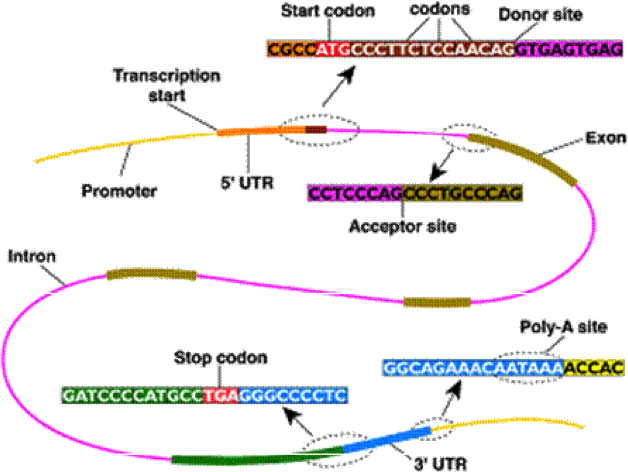
\includegraphics[width=\textwidth]{images/gene_feature}
  \end{columns}    
\end{frame}

%
\begin{frame}
  \frametitle{RNA features}
  \textcolor{hutton_blue}{RNA/ncRNA: characterised by complex secondary structure}
  \begin{columns}[T] 
    \column{.4\textwidth} 
      \begin{itemize}
        \item tRNA - transfer RNA
        \item rRNA - ribosomal RNA
        \item CRISPRs - prokaryotic defence, and genome editing
        \item many other functional classes, including enhancers
      \end{itemize}
    \column{.6\textwidth}
      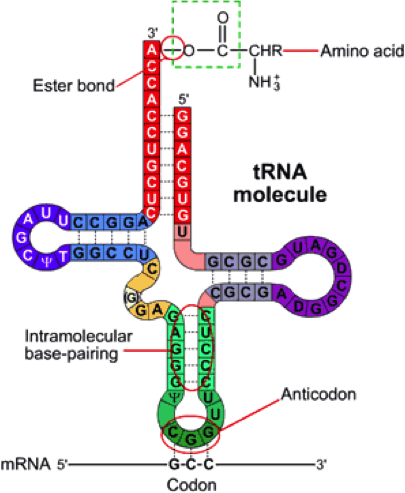
\includegraphics[height=0.7\textheight]{images/rna_feature}
  \end{columns}    
\end{frame}

%
\begin{frame}
  \frametitle{Gene features}
  \textcolor{hutton_green}{Regulatory sites:}
  \begin{itemize}
    \item transcription start sites (TSS)
    \item RNA polymerase (RNAp) binding sites
    \item transcription factor binding sites (TFBS)
    \item core, proximal and distal promoter regions
  \end{itemize}
  	
  \includegraphics[width=\textwidth]{images/_feature}
  \end{columns}    
\end{frame}

%
\begin{frame}
  \frametitle{Gene features}
  \textcolor{hutton_blue}{Genes:}
  \begin{columns}[T] 
    \column{.4\textwidth} 
      \begin{itemize}
        \item translation start
        \item introns
        \item exons
        \item translation stop
        \item translation terminator
      \end{itemize}
    \column{.6\textwidth}
      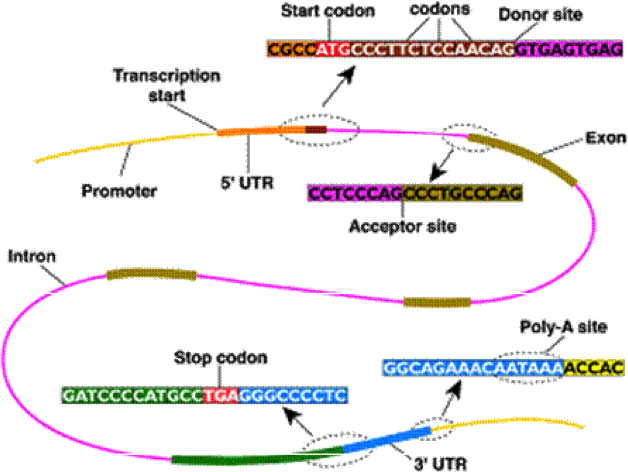
\includegraphics[width=\textwidth]{images/gene_feature}
  \end{columns}    
\end{frame}
% SUBSECTION
% Genome features
\subsection{Feature Finding}
%% feature_finding.tex
%% Author: Leighton Pritchard
%% Copyright: James Hutton Institute
%% Finding genome features

%
\begin{frame}
  \frametitle{Gene finding
  \footnote{\tiny{\href{http://dx.doi.org/10.1101/gr.088997.108
}{Liang \textit{et al.} (2009) \textit{Genome Res.} doi:10.1101/gr.088997.108
}}}
    \footnote{\tiny{\href{http://dx.doi.org/10.1038/nbt0807-883
}{Brent (2007) \textit{Nat. Biotech.} doi:10.1038/nbt0807-883
}}}
    \footnote{\tiny{\href{http://dx.doi.org/10.1186/1471-2105-5-59
}{Korf (2004) \textit{BMC Bioinf.} doi:10.1186/1471-2105-5-59
}}}
    }
  At genome scales, we need to automate functional prediction \\~\\    
  \textcolor{hutton_green}{Empirical (evidence-based) methods:}
  \begin{itemize}
    \item Inference from known protein/cDNA/mRNA/EST sequence
    \item Interference from mapped RNA reads (e.g. RNAseq)
  \end{itemize}
  \textcolor{hutton_blue}{\textit{Ab initio} methods:}
  \begin{itemize}
    \item Prediction on the basis of gene features (TSS, CpG islands, Shine-Dalgarno sequence, stop codons, nucleotide composition, etc.)
  \end{itemize}
  \textcolor{hutton_purple}{\textbf{Inference from genome comparisons/sequence conservation}}
\end{frame}

%
\begin{frame}
  \frametitle{Regulatory element finding
  \footnote{\tiny{\href{http://dx.doi.org/10.1186/1471-2105-12-238
}{Zhang \textit{et al.} (2011) \textit{BMC Bioinf.} doi:10.1186/1471-2105-12-238
}}}
    \footnote{\tiny{\href{http://dx.doi.org/10.1093/nar/gkt1123
}{Kilic \textit{et al.} (2013) \textit{Nucl. Acids Re.} doi:10.1093/nar/gkt1123
}}}
    \footnote{\tiny{\href{http://dx.doi.org/10.1016/j.gde.2005.05.002
}{Vavouri \& Elgar (2005) \textit{Curr. Op. Genet. Deve.} doi:10.1016/j.gde.2005.05.002
}}}
    }
  \textcolor{hutton_green}{Empirical (evidence-based) methods:}
  \begin{itemize}
    \item Inference from protein-DNA binding experiments
    \item Interference from co-expression
  \end{itemize}
  \textcolor{hutton_blue}{\textit{Ab initio} methods:}
  \begin{itemize}
    \item Identification of regulatory motifs (profile/other methods; TATA, $\sigma$-factor binding sites, etc.)
    \item Statistical overrepresentation of motifs
    \item Identification from sequence properties
  \end{itemize}
  \textcolor{hutton_purple}{\textbf{Inference from genome comparisons/sequence conservation}}
\end{frame}

%
\begin{frame}
  \frametitle{Multiple genome alignment}
  \Large{
    \textcolor{hutton_blue}{
      \textbf{
      EXERCISE 7: \\
      {\small \href{https://github.com/widdowquinn/Teaching-2015-03-17-UoD_compgenvis/blob/master/exercises/predict_CDS/bacterial_CDS_prediction.md}{\texttt{predict\_CDS/bacterial\_CDS\_prediction.md}}}
      }
    }
  }
\end{frame}

%
\begin{frame}
  \frametitle{Genecalling software}
  \textcolor{hutton_green}{Many options for this, including$\ldots$}
  \textcolor{hutton_blue}{Prokaryotes}
  \begin{itemize}
    \item Glimmer: {\tiny\href{http://ccb.jhu.edu/software/glimmer/index.shtml}{http://ccb.jhu.edu/software/glimmer/index.shtml}}
    \item GeneMarkS: {\tiny\href{http://opal.biology.gatech.edu/}{http://opal.biology.gatech.edu/}}
    \item RAST: {\tiny\href{http://rast.nmpdr.org/}{http://rast.nmpdr.org/}}
    \item BASys: {\tiny\href{https://www.basys.ca/}{https://www.basys.ca/}}
    \item \textbf{Prokka: {\tiny\href{http://www.vicbioinformatics.com/software.prokka.shtml}{http://}www.vicbioinformatics.com/software.prokka.shtml}}
  \end{itemize}
  \textcolor{hutton_purple}{Eukaryotes}
  \begin{itemize}
    \item GlimmerHMM: {\tiny\href{http://ccb.jhu.edu/software/glimmerhmm/}{http://ccb.jhu.edu/software/glimmerhmm/}}
    \item GeneMarkES: {\tiny\href{http://opal.biology.gatech.edu/gmseuk.html}{http://opal.biology.gatech.edu/gmseuk.html}}
    \item Augustus: {\tiny\href{http://augustus.gobics.de/}{http://augustus.gobics.de/}}
    \item SNAP: {\tiny\href{http://korflab.ucdavis.edu/software.html}{http://korflab.ucdavis.edu/software.html}}
  \end{itemize}
\end{frame}

%
\begin{frame}
  \frametitle{Feature identification}
  \textcolor{hutton_green}{All prediction methods give you errors}
  \begin{itemize}
    \item \textbf{False positive}: predicts features where there are none
    \item \textbf{False negative}: fails to predict a feature that is present
    \item \textbf{Magnitude}: does not identify correct bounds on/value for feature
    \item \textbf{Category}: predicts a feature to belong to the wrong class
  \end{itemize}
  \textcolor{hutton_blue}{All experiments have errors} \\~\\
  \textcolor{hutton_purple}{\textbf{Genome comparisons can help correct for these errors}}
\end{frame}
% SUBSECTION
% Who let the -logues out?
\subsection{Who Let the -logues Out?}
%% logues.tex
%% Author: Leighton Pritchard
%% Copyright: James Hutton Institute
%% Who let the -logues out?

%
\begin{frame}
  \frametitle{Who let the -logues out?}
  \Large{
    \textcolor{olive}{
      \textbf{
      Genome features can have complex evolutionary relationships \\~\\
      We need precise terms to describe these relationships
      }
    }
  }
  \begin{center}
    
\includegraphics[width=0.4\textwidth]{images/who_let_the_dogs_out}
  \end{center}      
\end{frame}

%
\begin{frame}
  \frametitle{The -logues drop
  \footnote{\tiny{\href{http://dx.doi.org/10.2307/2412448
}{Fitch \textit{et al.} (1970) \textit{Syst. Zool.} doi:10.2307/2412448
}}}
  }
  How do we understand the relationships between features in more than one genome?
  \begin{itemize}
    \item \textcolor{hutton_green}{Functional similarity}: \textbf{analogy}
    \item \textcolor{hutton_blue}{Evolutionary common origin}: \textbf{homology, orthology, etc.}
    \item \textcolor{hutton_purple}{Evolutionary/functional/family relationship}: \textbf{paralogy}
  \end{itemize}
  \begin{center}
    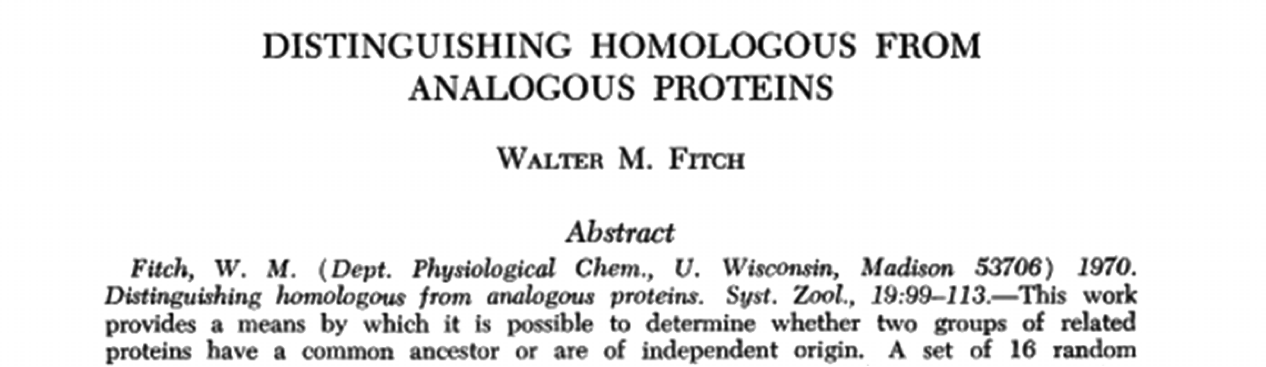
\includegraphics[width=\textwidth]{images/fitch}
  \end{center}    
\end{frame}

%
\begin{frame}
  \frametitle{Definitions
  }
  Technical terms describing evolutionary relationships
  \begin{itemize}
    \item \textbf{\textcolor{hutton_blue}{Homologues}}: share a common ancestor \textcolor{red}{\textbf{NOTE: there are NOT degrees of homology}}
    \item \textbf{\textcolor{hutton_blue}{Analogues}}: are functionally similar. Analogues may or may not share common ancestry
    \item \textbf{\textcolor{hutton_green}{Orthologues}}: are homologues that \textit{diverged through speciation}
    \item \textbf{\textcolor{hutton_purple}{Paralogues}}: are homologues that \textit{diverged through duplication} within the same genome
  \end{itemize}
  (also \textit{co-orthologues}, \textit{xenologues}, etc.)
\end{frame}
% SUBSECTION
% Finishing the Hat
\subsection{Finishing the Hat}

%%%
% LICENCE FOR REUSE
%% licence.tex
%% Author: Leighton Pritchard
%% Copyright: James Hutton Institute
%% These slides describe the licence for reuse of these slides and
%% materials

%
\begin{frame}
  \frametitle{Licence: CC-BY-SA}
  By: Leighton Pritchard \\[0.5cm]
  This presentation is licensed under the Creative Commons Attribution ShareAlike license \\
  \href{https://creativecommons.org/licenses/by-sa/4.0/}{https://creativecommons.org/licenses/by-sa/4.0/}
\end{frame}

% etc
\end{document}